\documentclass{beamer}
\usefonttheme[onlymath]{serif}

\usepackage[utf8]{inputenc}
\usepackage[T1]{fontenc}
\usepackage{lmodern}
\usepackage[francais]{babel}

% For table
\usepackage{booktabs} % To thicken table lines
\usepackage{multirow}
\usepackage{amsmath}

\usepackage[group-separator={,}]{siunitx}

  %for tikz figure
\usepackage{tikz}
\usetikzlibrary{decorations.pathreplacing}
\usetikzlibrary{fadings}
\usetikzlibrary{positioning} %for lstm
\usetikzlibrary{shapes, backgrounds}
\usetikzlibrary{arrows}
\usetikzlibrary{chains}
\tikzstyle{line} = [draw, -latex']
\usepackage{adjustbox}

\usepackage{pgfplots}
\usepackage{pgfplotstable}

\definecolor{color3}{rgb}{0,0.7,0.3}
\definecolor{color1}{rgb}{0,0.1,0.8}
\definecolor{color2}{rgb}{0.9,0.0,0}

\graphicspath{{img/}}


\mode<presentation> {
	\usetheme{ulaval}
	\setbeamercovered{invisible}
}

\logo{
	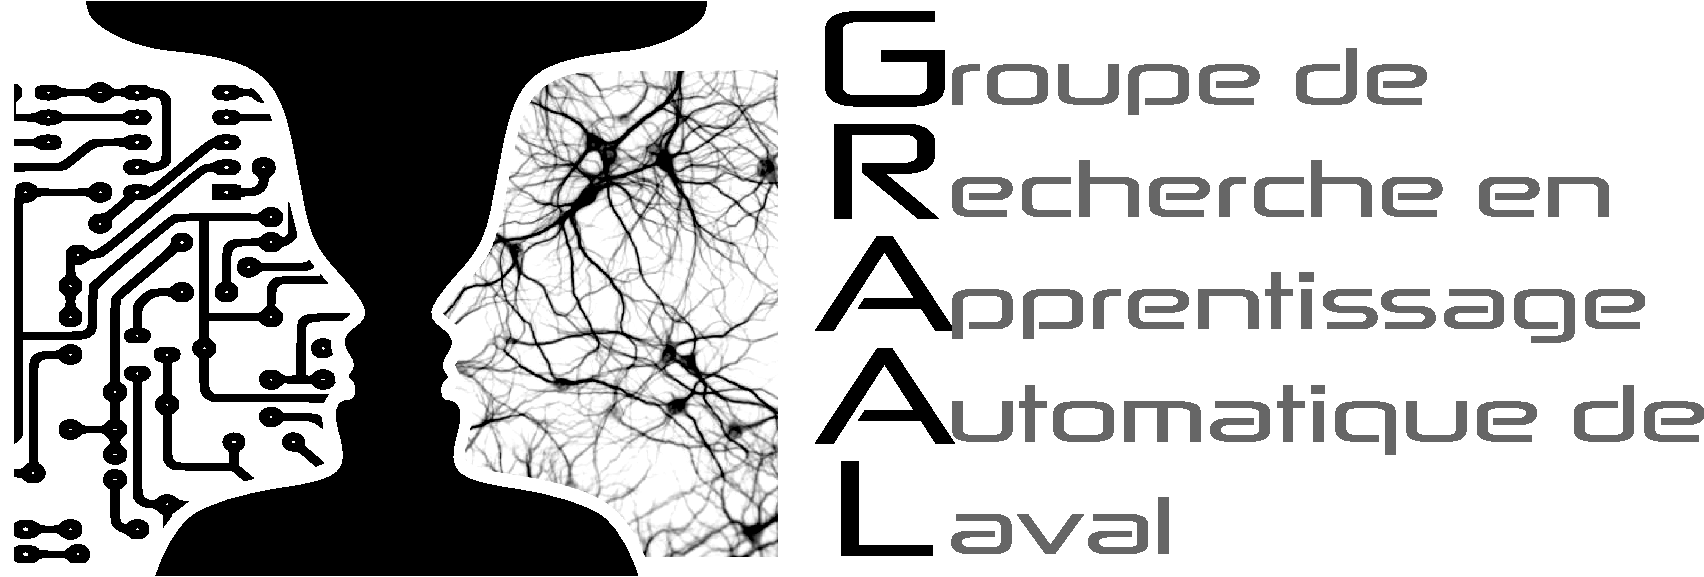
\includegraphics[height=0.65cm, keepaspectratio]{graal.pdf}\hspace{.2cm}\vspace{.85\paperheight}}


\title{Detection of Duplicates Among Non-structured Data From Different Data Sources}
%\subtitle[]{}

\author[D. Beauchemin]{David Beauchemin}
\institute[Université Laval]
{
	Département d'informatique et de génie logiciel, \\
	Université Laval\\
	\medskip
	{\emph{david.beauchemin.5@ulaval.ca}}
}
\date{28 july 2020}

\AtBeginSection[]
{
	\begin{frame}<beamer>
		\frametitle{Plan}
		\tableofcontents[currentsection]
	\end{frame}
}

\begin{document}
	
	
	\begin{frame}[label=titre, plain]
		\titlepage
		\begin{center}
			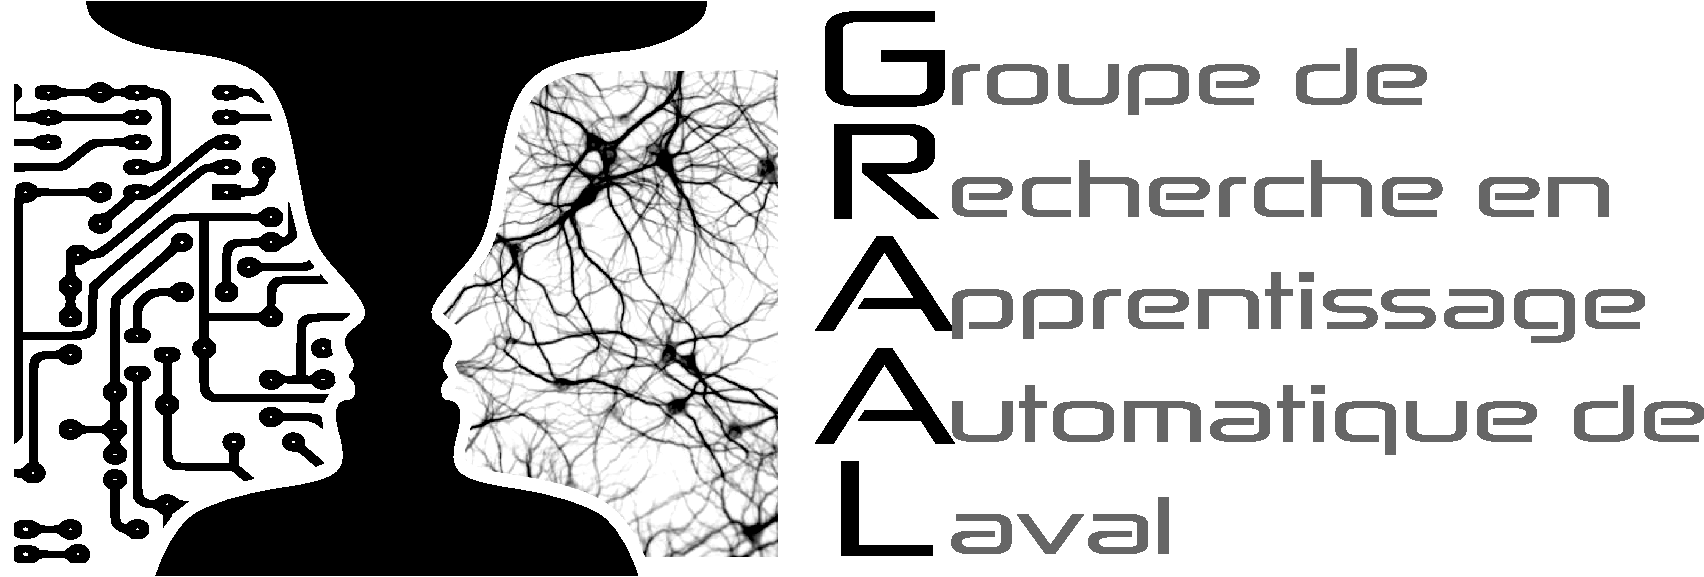
\includegraphics[height=1cm]{graal}
			
\includegraphics[height=1cm]{UL_P}
		\end{center}
	\end{frame}
	
	\section{Introduction}	
	
	\begin{frame}{Situation}
		When assessing a commercial risk, an insurer needs to gather various information about the risk. This long and complex process implies numerous questions. Thus an insurer is prompt to use an external source to help reduce the number of questions.
		\\\bigskip
		\uncover<2->{Thus, we want to detect duplicate of commercial risk in another data source using as little as possible information.}
		
		\uncover<3->{\begin{block}{Example}
				David Beauchemin, the owner of "Beauchemin inc.", calls for insurance. Using minimal information, we want to retrieve as much as possible from an external source to ask him as less than the necessary number of questions.
		\end{block}}
	\end{frame}
	
	\begin{frame}{How do we detect duplicate?}
		\only<1>{\begin{center}
			\begin{tikzpicture}[internal/.style={draw, rectangle, minimum width=4cm, inner sep=4pt},
			every text node part/.style={align=center}]
			\node[internal, align=center, minimum height=1.15cm](node1) at (-5, -2.75) {Duplicate \\ Detection Model};
			
			\node (node2) at (-1, -2.75) [cylinder, shape border rotate=90, draw, minimum height=1.15cm, minimum width=2cm, aspect=0.2] {Database 2};
			\draw[->,>=stealth] (node2) edge (node1.east);
			
			\node (node3) at (-9, -2.75) [cylinder, shape border rotate=90, draw, minimum height=1.15cm,minimum width=2cm, aspect=0.2] {Database 1};
			\draw[->,>=stealth] (node3) edge (node1.west);
			
			\node[internal, align=center, rounded corners=1ex, minimum height=1.15cm](node4) at (-5, -4.5) {\\};
			\node[internal, align=center, rounded corners=1ex, minimum height=1.15cm, fill=white](node5) at (-5.25, -4.75) {\\};
			\node[internal, align=center, rounded corners=1ex, minimum height=1.15cm, fill=white](node6) at (-5.50, -5) {Laval University};

			\draw[->,>=stealth] (node1) edge (node4);
			\end{tikzpicture}
		\end{center}}
	\only<2>{\begin{center}
			\begin{tikzpicture}[internal/.style={draw, rectangle, minimum width=4cm, inner sep=4pt},
			every text node part/.style={align=center}]
			\node[internal, align=center, minimum height=1.15cm](node1) at (-5, -2.75) {Duplicate \\ Detection Model};
			
			\node (node2) at (-1, -2.75) [cylinder, shape border rotate=90, draw, minimum height=1.15cm, minimum width=2cm, aspect=0.2] {Database 2};
			\draw[->,>=stealth] (node2) edge (node1.east);
			
			\node (node3) at (-9, -2.75) [cylinder, shape border rotate=90, draw, minimum height=1.15cm,minimum width=2cm, aspect=0.2] {Database 1};
			\draw[->,>=stealth] (node3) edge (node1.west);
			
			\node[internal, align=center, rounded corners=1ex, minimum height=1.15cm, fill=white](node6) at (-5, -4.5) {Laval University};
			
			\draw[->,>=stealth] (node1) edge (node6);
			\end{tikzpicture}
	\end{center}}
		\only<2->{Moreover, we consider only the top 1 document as the potential candidate.}
	\end{frame}

	\begin{frame}{How do we detect duplicate?}
		To detect duplicate we need the following \cite{christen2012data} 
		\begin{itemize}
			\item databases (at least two) (section 2),
			\item a way to determine the similarity between two documents (section 3).
		\end{itemize}
	\end{frame}
	
	\section{Databases}
	\subsection{\textit{Registre des Entreprises du Québec} (REQ)}
	
	\begin{frame}[label=REQ]\frametitle{\textit{Registre des Entreprises du Québec} (REQ)} 
		\begin{itemize}
			\item<1-> $\sim$3.5 millions entries \cite{contenureq}
			\begin{itemize}
				\item Names
				\item Address
				\item Economic activities
				\item Administrative informations
			\end{itemize}
		\end{itemize}
	\end{frame}
	
	\subsection{Private Dataset}
	\begin{frame}[label=intact]\frametitle{Private Dataset} 
		\begin{itemize}
			\item<1-> \num{21444} enterprises
			\begin{itemize}
				\item Name
				\item Address
				\item Economic activity
			\end{itemize}
		\end{itemize}
	\end{frame}
	
	\begin{frame}[label=intact-REQ]\frametitle{Private Dataset and the REQ} 
		\begin{itemize}
			\item<1-> \num{11649} commercial risk are in the province of Quebec.
			\begin{itemize}
				\item<2-> \num{1706} were annotated
				\begin{itemize}
					\item<3->  \num{1418} \textit{(commercial risk, REQ entity)}
					\item<3->  288 \textit{(commercial risk, None)}
				\end{itemize}
			\end{itemize}
			\item<4-> We only use the name and the address.
		\end{itemize}
	\end{frame}
	
	\begin{frame}\frametitle{Name} 
    	We have used two versions of the name.
		\begin{enumerate}
			\item<1-> Normalize name (NN): lowercase, whitespace and accent trimming.
			\begin{block}{Normalize Name}
				\begin{center}
					L'Université Laval $\Rightarrow$ \textit{l'universite laval}
				\end{center}
			\end{block}
			\item<2-> No stop words name (NSWN): stop words trimming (i.e \textit{le}, \textit{la}, \textit{de}) \cite{NLP-book-stop-word}.
			\begin{block}{No Stop Word Name}
				\begin{center}
					l'universite laval $\Rightarrow$ \textit{'universite laval}
				\end{center}
			\end{block}
		\end{enumerate}
	\end{frame}
	
	\begin{frame}[label=pretraitement-adresse]\frametitle{Address} 
		We also use two versions of the address.
		\begin{enumerate}
			\item<1-> Complete Address Normalize (NA): same as the name.
			\begin{block}{Complete Address Normalize}
				\begin{center}
					2325 rue de l'Université, Québec, QC, G1V 0A6 \\ $\Downarrow$ \\ \textit{2325 rue de l'universite, quebec, qc, g1v 0a6}
				\end{center}
			\end{block}
			\item<2-> Address components (AC): parsed and grouped by address components \cite{yassine2020leveraging}.
			\begin{block}{Address components}
				\begin{center}
					\scriptsize
					\begin{tabular}{cccc}
						\textbf{Civic Number} & 2325                 & \textbf{Unit Number} & $\emptyset$ \\
						\textbf{Street Name}  & rue de l'universite, & \textbf{Postal Code}    & g1v 0a6\\
						\textbf{Orientation}    & $\emptyset$                & &     \\
					\end{tabular}
				\end{center}
			\end{block}
		\end{enumerate}
	\end{frame}
	
	\section{Similarity Between Two Entities}
	
	\subsection{Similarity Algorithm}
	\begin{frame}[label=sim]\frametitle{Similarity Algorithm}	
		\begin{center}
			\begin{tikzpicture}[internal/.style={draw, rectangle, minimum width=3cm, minimum height=1.15cm, inner sep=4pt},
			every text node part/.style={align=center}]
			\node[internal, align=center](node1) at (-5, -2.75) {Similarity Algorithm};
			
			\node[internal, align=center, rounded corners=1ex, minimum height=1.15cm](node2) at (-0.75, -2.75) {Montreal \\ University};
			\draw[->,>=stealth] (node2) edge (node1.east);
			
			\node[internal, align=center, rounded corners=1ex, minimum height=1.15cm](node3) at (-9.25, -2.75) {Laval \\ University};
			\draw[->,>=stealth] (node3) edge (node1.west);
			
			\node[align=center](node4) at (-5, -4.5) {0.55};
			
			\draw[->,>=stealth] (node1) edge (node4);
			\end{tikzpicture}
		\end{center}
	\uncover<2->{Their similarity ranks the documents, and we select the best one as the duplicate candidate.}
	\end{frame}

	\begin{frame}\frametitle{Similarity Algorithm}
        Similarities algorithms are one that measures the resemblance between two string base on the distance between their tokens. \\\bigskip

        10 different algorithms were used.
	\end{frame}

	\begin{frame}\frametitle{Similarity Algorithms}
		\begin{block}{Jaccard Similarity}	
			\begin{equation*}
			\text{Jaccard}(\text{A, B}) =
			\begin{cases}
			0 & \text{if } |\text{A} \cap \text{B}| = 0 \text{ or } |\text{A} \cup \text{B}| = 0\\
			\frac{|\text{A} \cap \text{B}|}{|\text{A} \cup \text{B}|} & \text{otherwise}
			\end{cases}
			\end{equation*}
		\end{block}
		\begin{block}{Example}	
		\begin{center}
			Jaccard(Laval University, Montreal University)
			\bigskip\\ $\Downarrow$ \\ \bigskip
			$\frac{|\left\{\text{University}\right\}|}{|\left\{\text{University, Montreal, Laval}\right\}|} = \frac{1}{3} = \textbf{0,333}$
		\end{center}
		\end{block}
	\end{frame}

	\begin{frame}\frametitle{Similarity Algorithms}
		\begin{block}{String to String (StoS)}	
			\begin{equation*}
				\text{StoS}(\text{A, B}) =
				\begin{cases}
				1 & \text{if } \text{A}_i = \text{B}_j \ \forall i, j\\
				0 & \text{otherwise}
				\end{cases}
			\end{equation*}
		\end{block}
		\begin{block}{Example}	
			\begin{center}
				StoS(Laval University, Montreal University) $\Rightarrow$  0 \\
				StoS(Laval University, Laval University) $\Rightarrow$  1
			\end{center}
		\end{block}
	\end{frame}

	\begin{frame}\frametitle{Similarity Algorithms}
		\begin{block}{Jaro-Winkler}	
			\begin{equation*}
				\text{Jaro-Winkler}(\text{A, B}) = \text{Jaro}(\text{A, B}) + \frac{\min\left(P, 4\right)}{10} \times \left(1 - \text{Jaro}(\text{A, B})\right)
			\end{equation*}
		\end{block}
		\begin{block}{Example}	
			\begin{center}
				$\text{Jaro-Winkler(David, Daniel)} = \text{Jaro(David, Daniel)} + \frac{2}{10} \times  (1 - \text{Jaro(David, Daniel)})$\\ $\Downarrow$\\
				$0.7 + \frac{2}{10} \times 0.7 = 0.84$
			\end{center}
		\end{block}
	\end{frame}


	\begin{frame}\frametitle{Why Similarity Algorithm?}
		\begin{itemize}
			\item<1-> Easy to used
			\item<2-> No training
			\item<3-> Give good results
		\end{itemize}
	\end{frame}
	
	\begin{frame}\frametitle{Name Interesting Results \footnote{Positive examples only.}}
		\begin{table}[]
			\begin{tabular}{cccccc}
				\toprule
				& (\%)       & StoS   & Jaro  & Jaro-Winkler & Jaccard \\
				\midrule
				NN      & Accuracy & 41.47 & 63.40 & 63.47 & 65.73        \\
				NSWN & Accuracy & 44.15 & 64.46 & 65.23 & \textbf{66.50}    
				\\\bottomrule
			\end{tabular}
		\end{table}
		\begin{itemize}
			\item<1-> StoS give surprisingly good results considering the restrictive approach. 
			\item<2-> Removing stop words (second line) gives the best results.
			\item<3-> The prefix similarity used by Jaro-Winkler improved results (more when using NSWN).
		\end{itemize}
	\end{frame}
	
	\begin{frame}\frametitle{Address Interesting Results \footnote{Positive examples only.}}
		\begin{table}[]
		\begin{tabular}{cccccc}
				\toprule
				& (\%)       & StoS   & Jaro  & Jaro-Winkler & CSS \\
				\midrule
				CAN      & Accuracy & 0.00 & 48.03 & 48.10 & 45.91        \\
				AC & Accuracy & 13.19 & 51.83 & 51.83 & \textbf{52.19}    
				\\\bottomrule
			\end{tabular}
		\end{table}
		\begin{itemize}
			\item<1-> StoS give poor results using the normalized address due to the unomalized standard of writing (e.g., "qc" VS "(quebec)" and order of components).
			\item<2-> Using the address components without considering the order of the components improved results (AC).
			\item<3-> The local similarity used by Jaro-Winkler did not improve results this time since an address is rarely defined by is prefix.
			\item<4-> CSS gets the best results ($14\%$ below the previous best results using Jaccard).
		\end{itemize}
	\end{frame}
	
	\begin{frame}\frametitle{Missing Addresses}
		Since $16\%$ ($270$) of the pair \textit{(commercial risk, REQ entity)} are missing a address, the results are under-evaluated. For example, the CSS accuracy without those pairs is at $62.74\%$ near $10\%$ higher. \\\bigskip
		
		Those missing addresses are due to the confidentiality policy of the REQ \cite{guidereq}.
	\end{frame}
	
	\begin{frame}\frametitle{Similarity Algorithm Summary}
		\begin{itemize}
			\item<1-> Using either name or address, the similarities algorithms allows us to find the matched entity around $50\%$ of the time. The leading approach been Jaccard using the name at near $67\%$.
			\item<2-> Using the NSWN or the AC helps improve the results over the normalized name or address.
			\item<3-> The missing addresses pull down the results.
			\item<4-> To use positive and negative examples, we need to use a decision function. Such as a similarity threshold, were similarity below the threshold are rejected (the results are not shown). 
		\end{itemize}
	\end{frame}
	
	\subsection{Machine Learning}

	\begin{frame}\frametitle{Machine Learning Similarity Algorithm}
		\begin{center}
			\begin{tikzpicture}[internal/.style={draw, rectangle, minimum width=3cm, minimum height=1.15cm, inner sep=4pt},
			every text node part/.style={align=center}]
			\node[internal, align=center](node1) at (-5, -2.75) {Name-Address \\ Information Vector \\ Generator};
			
			\node[internal, align=center, rounded corners=1ex, minimum height=1.15cm](node2) at (-0.75, -2.75) {Montreal \\ University, \\ 2900 blvd \\ Edouard-Montpetit, \\ Montreal, QC};
			\draw[->,>=stealth] (node2) edge (node1.east);
			
			\node[internal, align=center, rounded corners=1ex, minimum height=1.15cm](node3) at (-9.25, -2.75) {Laval \\ University, \\ 2325 Rue de \\ l'Université, \\ Quebec, QC};
			\draw[->,>=stealth] (node3) edge (node1.west);
			
			\node[internal, align=center](node5) at (-5, -5.25) {Machine Learning \\ Model};
			
			\draw[->,>=stealth] (node1) edge (node5);
			
			\node[align=center](node4) at (-5, -7) {0.55};
			
			\draw[->,>=stealth] (node5) edge (node4);
			\end{tikzpicture}
		\end{center}
	\end{frame}
	
	\begin{frame}\frametitle{Name-Address Information Vector Generator}
		We used the previous similarity algorithm to generate an information vector between two entities using the NSWN and the CA.
		\begin{block}{Example of an information vector}
			\resizebox{\textwidth}{!}{%	
				\begin{tabular}{ccccccc}
					StoS     & Levenshtein   & Jaro-Winkler & LCSP   & Jaccard & Cosinus   & -    \\\midrule
					0.00 & 0.15     &  0.25       & 0.35 & 0.15 & 0.15 & -  \\
					\cmidrule(lr){1-7}
					StoS     & Levenshtein  & Jaro  &LCSP   & Jaccard & Cosinus   & CSS   \\\midrule
					0.00  & 0.16  & 0.55       & 0.15 & 0.45 & 0.37 & 0.48 
				\end{tabular}
			} % end of scope of "\resizebox"  directive
		\end{block}
	\end{frame}

	\begin{frame}\frametitle{Machine Learning Algorithm}
		\begin{enumerate}
			\item Logistic regression
			\item Random Forest
			\item Multilayer Perceptron
		\end{enumerate}
	\end{frame}

	\begin{frame}\frametitle{Why Machine Learning?}
		\begin{itemize}
			\item Allow us to use the name and the address simultaneously
			\item Generalization capability
		\end{itemize}
	\end{frame}

	\begin{frame}\frametitle{Models' Training Steps}
		\begin{enumerate}
			\item Data preprocessing
			\item Hyperparameters grid search
			\item Model training
			\item Evaluation of the trained model for the duplicate detection task
		\end{enumerate}
	\end{frame}
	
	\begin{frame}\frametitle{Data preprocessing}
		\begin{itemize}
			\item<1-> 80-20 splitting of the data (\num{1706} annoted exemples).
			\item<2-> From the train dataset ($80\%$), we randomly match the negatives pair \textit{(commercial risk, None)} (241 examples) with a REQ entity.
			\item<3-> To balance the dataset (1364 positives vs. 241 negatives), we randomly select the first name and address of a REQ entity to create a fake commercial risk and randomly pair it with another REQ entity. Resulting in a training dataset of \num{2246} \textit{(commercial risk, REQ entity)} pair.
			\item<4-> We fit a standard scaler on the training dataset. With that standard scaler, we applied a transformation over all the vectors (train and test).
		\end{itemize}	
	\end{frame}

	\begin{frame}\frametitle{Hyperparameters Grid Search \& Model Training}
		\begin{itemize}
			\item A grid search for the logistic regression ($C$ and tolerance) and the random forest (number of estimators).
			\item A random search for the multilayer perceptron (number of layers and neurons and the tolerance).
			\item Cross-validation approach using a 5-folds.
		\end{itemize}	
		After the grid search, we retrain using the best parameters.
	\end{frame}
	
	\begin{frame}\frametitle{Evaluation}
		We evaluate our three trained models against the best configuration, Jaccard using the name, but reevaluated with the validation dataset ($20\%$ of the \num{1706} annotated examples). \\\bigskip
		
		We evaluated the algorithm with positives and negatives examples (for recall and precision). The decision function is a similarity threshold where a similarity below a numerical threshold (e.g., $0.7$) is rejected.\\\bigskip
		
		We aim to maximize the recall since our objective is to detect the more duplicate as possible since we can, later on, validate the duplicate manually. 
	\end{frame}

	\begin{frame}\frametitle{Results}
			\centering
			\begin{tabular}{cccc|c}
				\toprule
				(\%) &\begin{tabular}[c]{@{}c@{}}Logistic \\ Regression\end{tabular}  & \begin{tabular}[c]{@{}c@{}}Random \\ Forest\end{tabular} & \begin{tabular}[c]{@{}c@{}}Multilayer \\ perceptron\end{tabular} & Jaccard \\ \midrule
				Precision  & \textbf{89,77}                                                                                                                 & 81,06                                                  & 87,55                                                            & 81,78   \\
				Recall    & 66,67                                                                                                               & 73,54                                                   & \textbf{79,73}                                                            & 72,51  \\
				Accuracy & 64,91                                                                                                           & 62,87                                                    & \textbf{73,10}                                                           & 62,87   \\
				\bottomrule
			\end{tabular}
			\begin{itemize}
				\item<1-> The random forest and the multilayer perceptron achieve better recall than Jaccard. The best being the perceptron with near $80\%$ recall.
				\item<2-> The logistic regression achieves the lowest result even if the Jaccard similarity is used in the generation of the information vector.
		\end{itemize}
	\end{frame}

	\begin{frame}\frametitle{Example of an Error}
		\resizebox{\textwidth}{!}{%
			\begin{tabular}{cc}
				\toprule
				Commercial Risk                                                                     & Entity                                                                                                 \\\midrule
				construction alain cloutier inc.                                                       & construction steeve arbourd inc.                                                                       \\
				\begin{tabular}[c]{@{}c@{}}1030 rue de l'ardoise sherbrooke j1c 0j6\end{tabular} & \begin{tabular}[c]{@{}c@{}}2-1822 rue notre-dame, l'ancienne-lorette, g2e 3c7\end{tabular}\\\bottomrule
			\end{tabular}%
		}	
	\\\bigskip
		The following error was only generated with the logistic regression model. The algorithm matched the two with a similarity of 0.99934, even if the annotated duplicate appear with the same name and a slightly
		different address (similarity of ~0.998). 
	\end{frame}

	\begin{frame}\frametitle{Improving the Results}
		The previous error highlights a problem of our approach; so far, we have tried to match with \textbf{the} most similar, and the generated similarity are close to each other, making it restrictive to use only the best similarity.
		\\\bigskip
		Since our approach aims to prefill the information of an insurance application, we can return more than one and use a human validation to select the best one from $N$ possibilities.
	\end{frame}

	\begin{frame}\frametitle{$N$ Most Similar}
		We consider a matching is good when the pair \textit{(commercial risk, REQ entity)} is included in the $N$ most similar.
	\end{frame}

	\begin{frame}\frametitle{Results}
			\begin{tikzpicture}
			\begin{axis}[grid style={dashed,gray!50}, axis y line*=left, axis x line*=bottom, ybar, nodes near coords=\rotatebox{90}{\pgfmathprintnumber\pgfplotspointmeta}, nodes near coords style={font=\tiny}, every axis plot/.append style={line width=1.25pt, mark size=0pt}, width=\textwidth, height=.225\textwidth, grid=none, xtick=data, symbolic x coords={LR, RF, MP, Jaccard}, ylabel=Precision (\%), legend style={nodes={scale=0.8, transform shape},  at = {(0.45, 2.25)}, anchor = north}, legend columns=4]
			\addplot[color3, fill,  opacity=0.5] table[x=x3, y=y3, col sep=comma]{./data/plot_precision_top_n.csv};
			\addlegendentry{Top 1};
			\addplot[color1, fill,  opacity=0.5] table[x=x4, y=y4, col sep=comma]{./data/plot_precision_top_n.csv};
			\addlegendentry{Top 5};
			\addplot[color2, fill,  opacity=0.5] table[x=x5, y=y5, col sep=comma]{./data/plot_precision_top_n.csv};
			\addlegendentry{Top 10};
			\end{axis}
			\end{tikzpicture}
			\begin{tikzpicture}
			\begin{axis}[grid style={dashed,gray!50}, axis y line*=left, axis x line*=bottom, ybar, nodes near coords=\rotatebox{90}{\pgfmathprintnumber\pgfplotspointmeta}, nodes near coords style={font=\tiny}, every axis plot/.append style={line width=1.25pt, mark size=0pt}, width=\textwidth, height=.225\textwidth, grid=none, xtick=data, symbolic x coords={LR, RF, MP, Jaccard}, ylabel=Recall (\%)]
			\addplot[color3, fill,  opacity=0.5] table[x=x6, y=y6, col sep=comma]{./data/plot_rappel_top_n.csv};
			\addplot[color1, fill,  opacity=0.5] table[x=x7, y=y7, col sep=comma]{./data/plot_rappel_top_n.csv};
			\addplot[color2, fill,  opacity=0.5] table[x=x8, y=y8, col sep=comma]{./data/plot_rappel_top_n.csv};
			\end{axis}
			\end{tikzpicture}
			\begin{tikzpicture}
			\begin{axis}[grid style={dashed,gray!50}, axis y line*=left, axis x line*=bottom, ybar, nodes near coords=\rotatebox{90}{\pgfmathprintnumber\pgfplotspointmeta}, nodes near coords style={font=\tiny}, every axis plot/.append style={line width=1.25pt, mark size=0pt}, width=\textwidth, height=.225\textwidth, grid=none, xtick=data, symbolic x coords={LR, RF, MP, Jaccard}, ylabel=Accuracy (\%)]
			\addplot[color3, fill, opacity=0.5] table[x=x0, y=y0, col sep=comma]{./data/plot_exactitude_top_n.csv};
			\addplot[color1, fill, opacity=0.5] table[x=x1, y=y1, col sep=comma]{./data/plot_exactitude_top_n.csv};
			\addplot[color2, fill, opacity=0.5] table[x=x2, y=y2, col sep=comma]{./data/plot_exactitude_top_n.csv};
			\end{axis}
			\end{tikzpicture}
	\end{frame}
	
	\begin{frame}\frametitle{Results}
		\begin{itemize}
			\item Using a top $N$ approach greatly improved the results. 
			\item Using $N = 10$, we can achieve a near max recall at $~91\%$ with the multilayer perceptron (max of $93\%$ with the indexing).
		\end{itemize}
	\end{frame}	

	\begin{frame}\frametitle{Inference Times}
		\centering
		\begin{tabular}{cccc|c}
			\toprule
			(second) & \begin{tabular}[c]{@{}c@{}}Logistic\\ Regression\end{tabular} & \begin{tabular}[c]{@{}c@{}}Random\\ Forest\end{tabular} & \begin{tabular}[c]{@{}c@{}}Multilayer \\ Perceptron\end{tabular} & Jaccard \\\midrule
			\begin{tabular}[c]{@{}c@{}}Time\end{tabular} & 1,32                                                            & 1,74                                                       & 1,34                                                        & 0,25     \\\bottomrule
		\end{tabular}
	\end{frame}

	\begin{frame}\frametitle{Machine Learning Algorithm Summary}
		\begin{itemize}
		\item<1-> The used of name and address simultaneously with a machine learning algorithm improved the results.
		\item<2-> Using a top $ N $ approach helps achieve better results when $ N $ is greater than 1.
		\item<3-> Inference times (of machine learning models) are similar to using only a similarity algorithm.
		\end{itemize}
	\end{frame}
	
	\section{Conclusion}
	
	\begin{frame}\frametitle{Conclusion}
		\begin{itemize}
			\item We have shown that using a similarity algorithm can achieve good results.
			\item Uses of machine learning algorithm (such as multilayer perceptron) can achieve greater results.
			\item Using a $N$ most similar approach, where $N$ is greater than one, help improved the results, achieving almost the max recall value.
		\end{itemize}
	\end{frame}

	\begin{frame}\frametitle{Future Works}
		\begin{itemize}
			\item Word embeddings \cite{word2vec, glove, wu2017starspace, name2vec, singh2019embedding}
			\item Siamese Network \cite{godbole2018siamese, 8967103}
			\item Uses of spatial data \cite{10.1145/1183471.1183486}
			\item Removal of more specitif stop words using a TF-IDF approach \cite{tfidf}
		\end{itemize}
	\end{frame}

	\begin{frame}{Acknowledgment}
		\begin{itemize}
			\item This research was supported by the Natural Sciences and Engineering Research Council of Canada (IRCPJ 529529-17) and a Canadian insurance company. 
			\item Luc Lamontagne for his mentorship.
		\end{itemize}
	\end{frame}
	
	\begin{frame}[t, allowframebreaks]
		\frametitle{References}
		\bibliographystyle{apalike}
		\bibliography{DDANSDDDS}
	\end{frame}
	
\end{document}